\chapter{Fundamental Blocks of the Work} \label{chapter_two}

In the previous chapter I discussed the importance of Image Stabilization (Video Stabilization) and the challenges associated performing it using an IMU sensor. This chapter contains the image stabilization techniques available and also we make a case for our chosen technique. Then we will also discuss in depth the challenges associated with IMU pose-estimation and how we can overcome those challenges. Types of neural networks and their applications will also be briefly conferred as they are a huge part of this work.

\section{Image Stabilization}
\label{sec:image_stab}
If a camera is not stationary during video capture the output video quality may degrade and not look good. Depending on the movements during capture, video may look very shaky or even the subjects may not be properly visible. This is very undesirable and can cause visual discomfort \citep{jia2012probabilistic}. The solution to this maybe to keep the camera steady by mounting it on stable tripod or to a rigid object. But this is not practically possible all the time. There are various scenarios in which the camera may move around a lot and the movements may not be smooth at all e.g an action camera mounted on a helmet or a bicycle, a camera mounted on a car or a robot in wild or some move-able rig or a robot arm.

The motion of the camera can be high-frequency tremors due to vibration, shaking or jiggling of the mounting point \citep{ryu2012robust} or low frequency such as movement of handheld camera during walking \citep{dis_review}. Practically, in most of the video recording scenarios, the camera will have some movement. The goal of image stabilization is to create a output video with same visual content without the undesired movements. 

% Start: Image Stabilization
\subsection{Types of Image Stabilization}
To deal with such movements and to make the video stable various techniques exist. These techniques are grouped in two categories:

\begin{itemize}
\item Hardware Image Stabilization
\item Digital Image Stabilization  
\end{itemize}
There are techniques which combine both these methods and are called Hybrid Image Stabilization techniques.

The goal of each of these stabilization techniques is to estimate the motion or pose and then use the estimated motion to stabilize the video. Motion/pose estimation will be discussed in the section \ref{sec:pose_estimation} in detail.

\subsubsection{Hardware Image Stabilization (HIS)}
Hardware image stabilization at its core means moving the lens or the image sensor or the camera setup itself to counteract these movements while recording the video. The movements of camera can be minimised by the use of mechanical stabilizers like tripods or dollies \citep{5995525}. The use of electronic gimbals for video recording has also increased recently for both professionals and hobbyists. Video can also be stabilized by varying the optical path between lens and the image sensor. This is generally achieved by using electronic motors and IMU sensors to move around the lens or the image sensor or both to cancel out the motions. After the motions have been counter-acted upon, images are captured which results in a stabilized video output as seen in figure \ref{fig:his}. These methods although mostly effective are not perfect and have both advantages and disadvantages.

\begin{figure}[H]
\centering
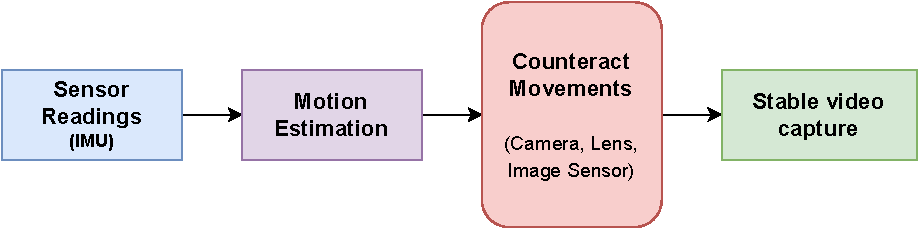
\includegraphics[scale=0.6]{images/fig_chapter2/2_1_his.pdf}
\caption{Hardware Image Stabilization}
\label{fig:his}
\end{figure}

\textbf{Advantages of HIS: }

\begin{itemize}
\item No post-processing for stabilization needed.
\item Works irrespective of the nature of object being captured.
\item Full image without cropping can be used.
\item Shutter Speed of the camera can be reduced
\end{itemize}

\textbf{Disadvantages of HIS:}
\begin{itemize}
\item Camera setups are very bulky.
\item These solutions can be very expensive.
\item More moving parts means higher maintenance.
\item Cannot be improved once hardware is implemented.
\item Not possible on all camera setups.
\end{itemize}

\subsubsection{Digital Image Stabilization (DIS)}
Digital Image Stabilization also called Digital Video Stabilization (DVS) is a software based image stabilization technique \citep{dis_review}. The technique here is similar what is done is HIS i.e. first motion of the camera is estimated (pose-estimation) and based on this, the image is stabilized. The difference here is that after pose estimation is done, instead of moving around the hardware a suitable transformation (warping) is applied to the image \citep{dis_feat_track} as shown is figure \ref{fig:dis}. The resulting stabilized image (video) is motionless irrespective of the camera motions. DIS is be a very powerful technique but like other methods and techniques, it has its advantages and disadvantages.

\begin{figure}[H]
\centering
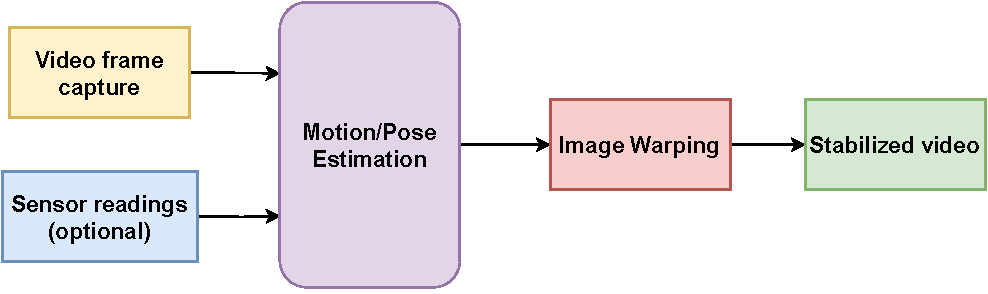
\includegraphics[scale=0.6]{images/fig_chapter2/2_1_dis.pdf}
\caption{Digital Image Stabilization}
\label{fig:dis}
\end{figure}

\textbf{Advantages of DIS: }
\begin{itemize}
\item Cost effective.
\item Smaller camera setups can be used.
\item No necessary changes need to be made to the camera setup for DIS.
\item Can be achieved using IMU sensors for pose estimation which are not very expensive.
\item Can be applied to any video; even the historic ones.
\item Different DIS algorithms can be used on a single video in post processing.
\item Relatively easy to modify DIS software.
\end{itemize}

\textbf{Disadvantages of DIS:}
\begin{itemize}
\item The resolution of the output images (video) is reduced (generally by 5 to 10 percent).
\item May require some manual labour (like in Adobe Premiere Pro: manual feature tracking).
\item Some videos are very difficult (even impossible) to stabilize if there is too much vibration or the features are not visible.
\item May require a lot of computational power (optical flow)
\end{itemize}

Now we know that for any type of image stabilization motion estimation is fundamental and this is what will be discussed in the next section of this report.

% Start: Motion Estimation
\section{Motion Estimation for Image Stabilization}
\label{sec:pose_estimation}
Camera motion (pose) estimation is very important and one of the most challenging parts of image stabilization. Before hardware and digital stabilization techniques/algorithms can be implemented, we need to perform pose estimation to figure out the camera motions. Then based on these camera motions we can stabilize a video. The accuracy of motion estimation ultimately determines the effectiveness of image stabilization \citep{ryu2012robust}. To estimate the camera motion many sensor based and software based techniques exist as show in figure \ref{fig:cam_pose_est}.

\begin{figure}[H]
\centering
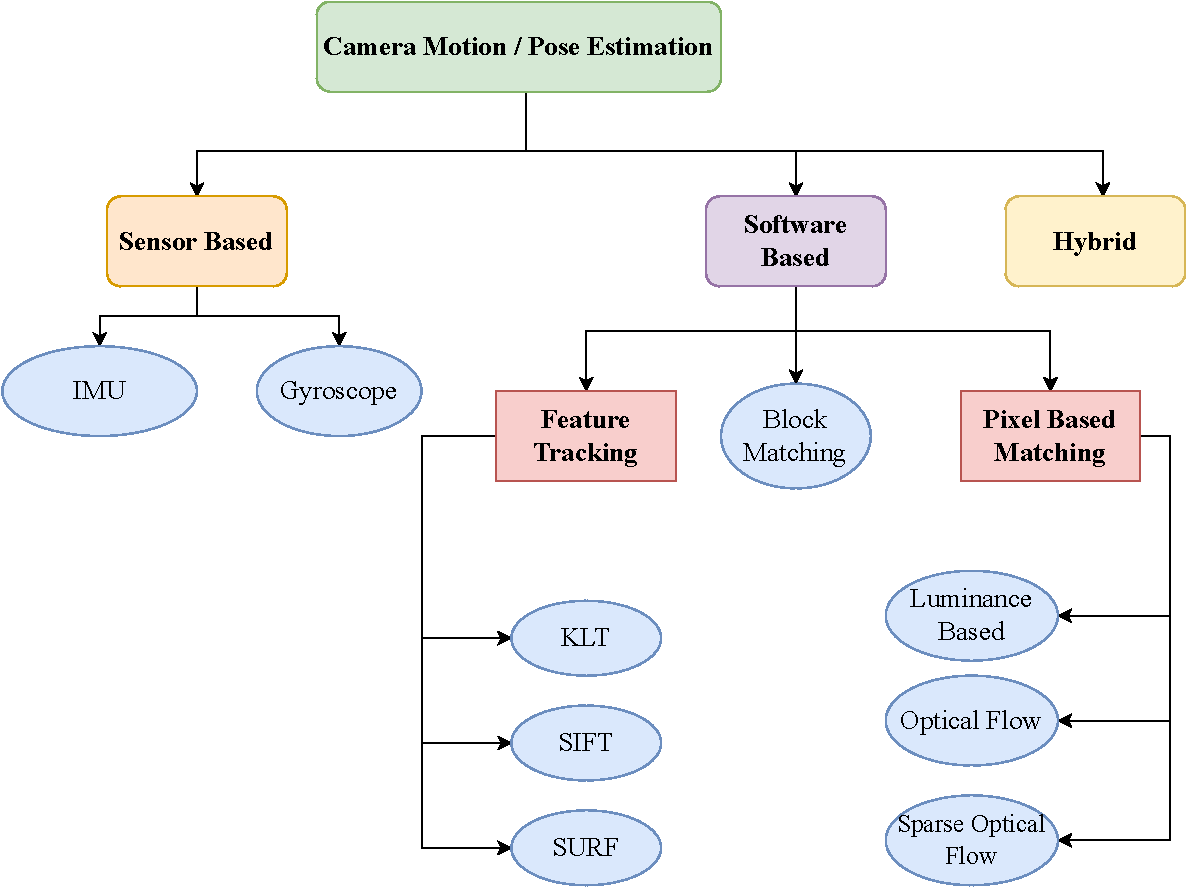
\includegraphics[scale=0.6]{images/fig_chapter2/cam_pose_estimation.pdf}
\caption{Camera Motion/Pose Estimation Techniques}
\label{fig:cam_pose_est}
\end{figure}


\subsection{Software based motion estimation techniques}
\label{sec:software_motion_estimation}
Software based motion estimation techniques/algorithms use the images (frames) coming from the camera for motion estimation and subsequently for stabilization. Some of these software based techniques are listed below \citep{dis_review}:

\begin{itemize}
\item Pixel-based matching
\item Block-Matching
\item Feature-Matching
\end{itemize}

Each of these approaches/algorithms used in motion estimation are briefly discussed in the subsequent sections. This will also lay a foundation for why we are not using any of these techniques for this work.

\subsubsection{Pixel-Based Matching}
This method estimates pose by determining the motion of pixels between two frames \citep{dis_review}. For correspondence determination, luminance of two consecutive frames is assumed to be constant throughout. This poses a problem and there can be many pixels having same luminance, so, other constraints are also needed to obtain a unique solution \citep{dis_review}. 

Finding  \textbf{\textit{Optical Flow}} between two consecutive frame is another method for motion estimation. Optical flow is the distribution of apparent velocities of movement of brightness patterns in an image \citep{horn1981determining}. This gives us important information about the spatial arrangement of the objects viewed and the rate of change of this arrangement \citep{gibson1977analysis}. Using this information, relative motions can be estimated between consecutive image frames. These relative motions can be used for camera motion estimation. Many modern neural network based optical flow algorithms have also been developed recently and are used in image stabilization tasks \citep{deep_opti_stab}. Although this method can give us good results, but, it has very high computational requirements and thus can be very slow.

\subsubsection{Block-Matching}
Block matching techniques use blocks of pixels for motion estimation instead of finding correspondence between pixels of consecutive frames. This allows to remove some ambiguities that occur in pixel-based matching methods \citep{dis_review}. Block-matching approach offers a flexible trade-off between complexity, computational efficiency and accuracy \citep{dis_review} but relies heavily on unambiguous features in the image.

\subsubsection{Feature-Matching (Tracking)}
In these methods, the algorithm first selects the features that are easily recognisable and distinguishable. The motion is estimated by tracking only these features, so, this make them computationally less expensive. There are several feature tracking algorithms that are widely used in many computer vision applications.

\paragraph{}\textbf{Kanade Lucas Tomasi (KLT) feature tracker} \citep{tomasi1991detection} is a widely used feature tracking algorithm in computer vision. Features are selected and their position is initialized using this technique and then optical flow is used to track their position \citep{dis_review}.

\paragraph{}\textbf{Scale-invariant feature transform (SIFT)} is also used for motion estimation in digital image stabilization algorithms.  It has been designed for extracting highly distinctive invariant features from images, which can be used to perform reliable matching of the same object or scene between different images \citep{battiato2007sift}. It contains the orientation of the feature in order to be rotation-invariant \citep{dis_review}.

\paragraph{}\textbf{Speeded up robust features (SURF)} is inspired by SIFT but is faster \citep{dis_surf}. This technique is also widely used in feature selection and tracking for motion estimation.

A common theme here in software based motion estimation techniques is to detect features (be it a pixel, or a group of pixels or any other particular image feature) and then tracking it for motion estimation. But, there are certain use cases like ours where feature tracking is very difficult or unreliable. The features in an image sequence can be moving in different directions, which makes reliable motion estimation using these techniques impossible. This is the case for this work and the goal is to \textit{estimate motion using technique which is image invariant}. To achieve this we decided to use sensor based pose-estimation techniques.

\subsection{Sensor based Motion Estimation}
Pose estimation is a huge are of research especially for the field of robotics and autonomous driving. There are various sensors like Accelerometers, Gyroscopes, Magnetometers and Satellite Navigation systems available. For camera pose estimation, generally Gyroscopes and Accelerometers are used. In combination, these two sensors are called \textit{Inertial Measure Unit (IMU) Sensors}. For this work, we will be using IMU for pose estimation as using it has many advantages and will make our image stabilization algorithm image invariant.

% Start: IMU Sensors
\section{Inertial Measurement Unit (IMU) Sensors}
\label{sec:imu}
IMU sensor is one of the most commonly used sensors in the world and present all around us in mobile devices, virtual reality gear and camera. It is very common to use IMU sensor for pose estimation. An IMU sensor measures acceleration(m/s²) and angular velocity (rad/s).  They can make these measurements in multiple degrees of freedom e.g., a 6-DoF IMU sensor includes a 3-axis accelerometer (x, y, z) and 3 axis gyroscope (x, y, z)  \citep{constant2021data}. The accelerometer will make independent acceleration measurements in these axis. Similarly, the gyroscope makes independent angular velocity measurements about these three axis.

IMU sensors are used in a wide variety of applications like navigation, robotics, drones, smart watches, sports learning, augmented reality systems, industrial quality control \citep{ahmad2013reviews}  and also for image stabilization in cameras. In all these applications, IMU sensor is used for pose estimation in some form; either for absolute pose estimation or change in pose.

There are a lot of reasons to use IMU sensors and these reasons are surely a very huge contributor to them being one of the most commonly used sensors in the world. Some of their qualities are \citep{woodman2007introduction}.:

\begin{itemize}
\item They have small size
\item low weight
\item rugged construction 
\item low power consumption 
\item cheap
\item high reliability 
\item low maintenance
\item can be used in hostile environments 
\end{itemize}

\subsection{Pose Estimation with IMUs}
Pose for any object is its position(x, y, z) and its orientation(yaw, pitch, roll) with respect to some reference coordinate system. To estimate pose of an object, we continuously take measurements from IMU and using some algorithm we estimate its pose. Figure \ref{fig:strapdown_imu} below shows the strap-down inertial navigation algorithm \citep{woodman2007introduction}. For orientation estimation gyroscope readings are used and for position estimation both gyroscope and accelerometer readings are used. The use of this algorithm directly for pose-estimation is not possible as the IMU readings are far from being ideal, they contain noise and have a bias \citep{woodman2007introduction} which needs to be accounted for.

\begin{figure}[H]
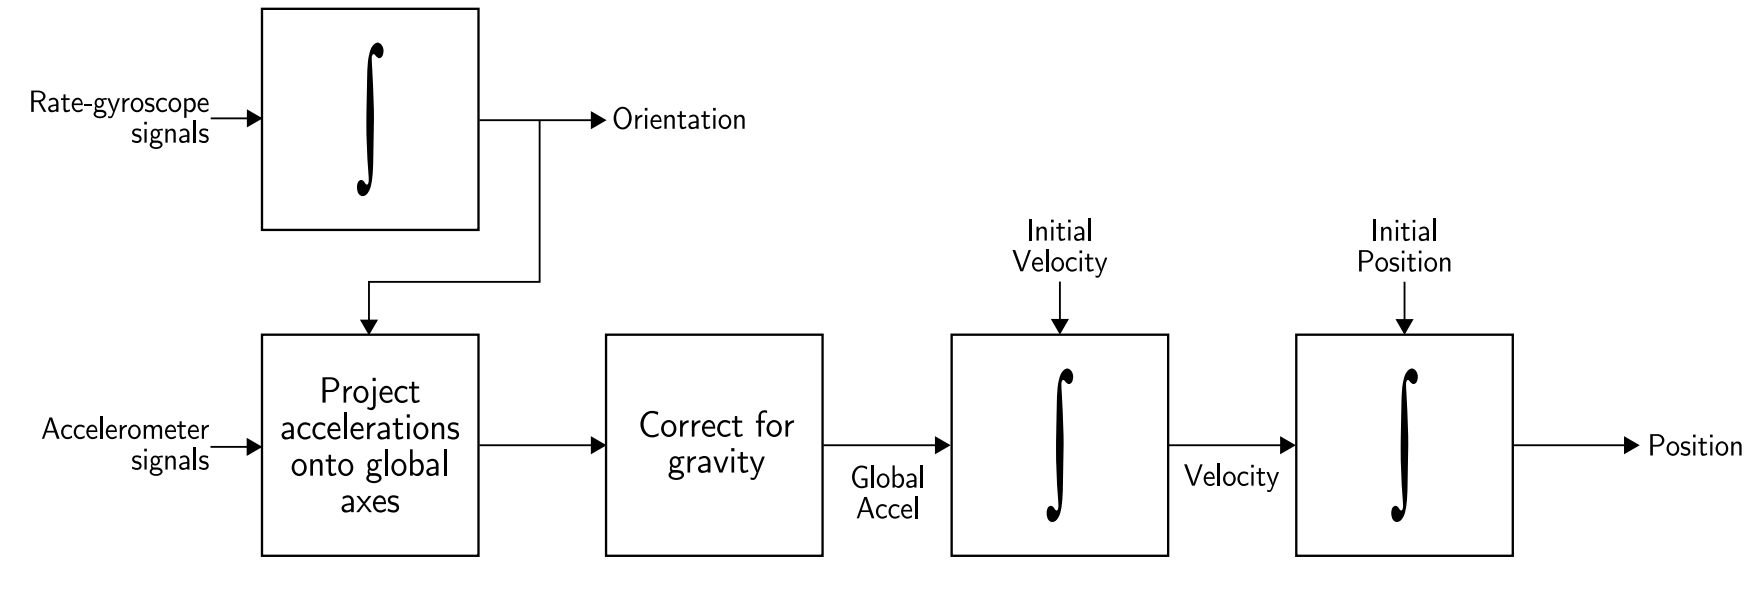
\includegraphics[scale=0.2]{images/fig_chapter2/strap_imu_algo.png}
\caption{Strap-down inertial navigation algorithm \citep{woodman2007introduction}}
\label{fig:strapdown_imu}
\end{figure}

\subsection{IMU Noise Models}
MEMS sensor outputs are inherent to noise and there is different types of noise with which we have to deal. For IMUs, the readings coming from a sensor could be modelled as a combination of three entities: true signal, bias and white noise.

\textbf{Gyroscope}
\begin{equation}
    \omega_{n}(t) = \omega(t) + b_{g}(t) + n_{g}
\label{eqn:gyro_noise}
\end{equation}

Where $ \omega_{n}(t) $ is the noisy gyroscope signal, $ \omega(t) $ is the true gyroscope signal, $ b_{g}(t) $ is the gyroscope bias and $ n_{g} $ is the gyroscope white noise.

\textbf{Accelerometer}
\begin{equation}
    a_{n}(t) = a(t) + b_{a}(t) + n_{a}
\label{eqn:accel_noise}
\end{equation}

Where $ a_{n}(t) $ is the noisy accelerometer signal, $ a(t) $ is the true accelerometer signal, $ b_{a}(t) $ is the accelerometer bias and $ n_{a} $ is the accelerometer white noise.


To visualise the \textit{Noise Model}, let's take a true unit signal as show in figure \ref{fig:imu_noise}. \textbf{Bias} can be defined as constant offset from true signal value. White noise can be thought of as random fluctuations of equal intensity and different frequency from the true value of the signal (\ref{fig:imu_noise}).

\begin{figure}[H]
  \begin{subfigure}{\linewidth}
  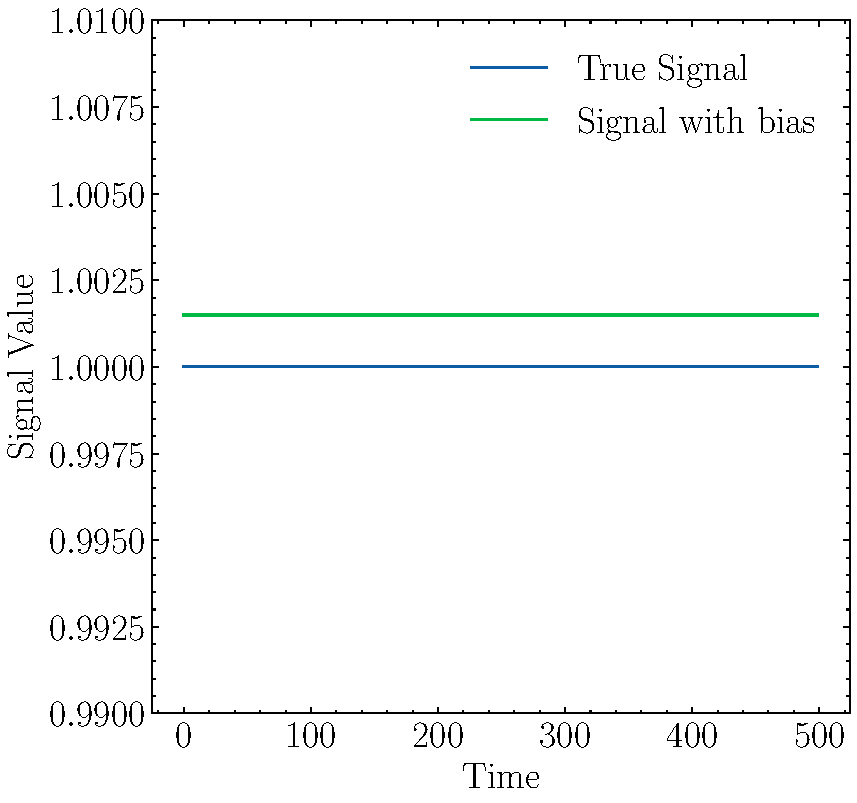
\includegraphics[width=.5\linewidth]{images/fig_chapter2/noise_figs/signal_with_bias.pdf}\hfill
  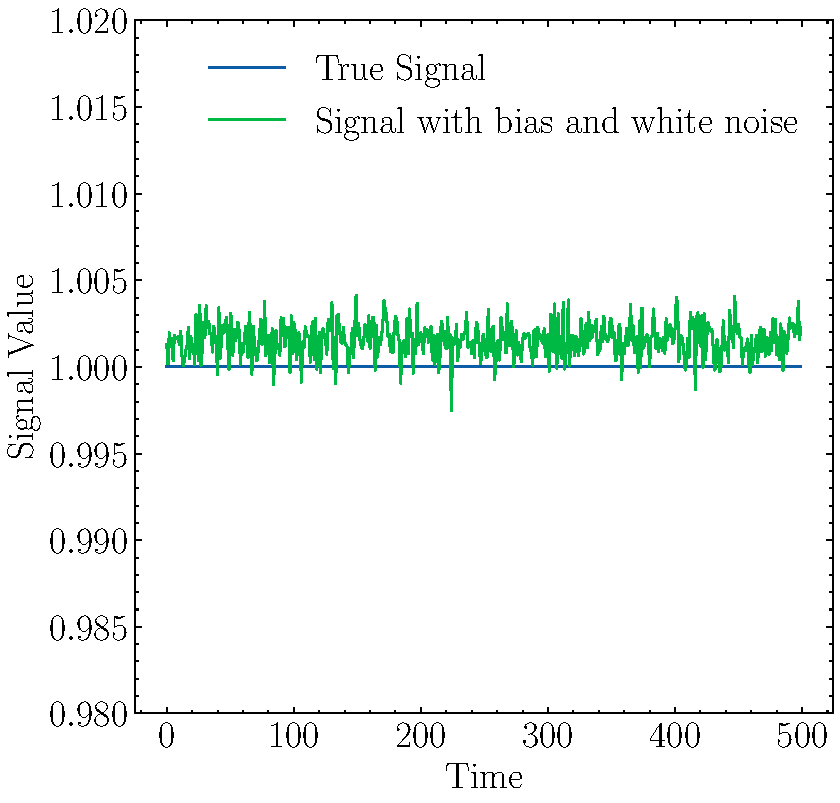
\includegraphics[width=.5\linewidth]{images/fig_chapter2/noise_figs/signal_with_bias_and_noise.pdf}
  \end{subfigure}\par\medskip
  \caption{IMU Noise Model Visualisation}
\label{fig:imu_noise}
\end{figure}

For both gyroscope and accelerometer the signal can be independently modeled this way in each of its axis (x, y and z) \citep{imu_noise}. As you can see from the plots, the noisy signal looks very different from the true signal. Using the noisy signal directly for pose estimation can lead to very inaccurate results. Although the modelling equation looks the same for both gyroscope and accelerometer, but they have different effects on pose estimation as the strap-down inertial algorithm suggests. So, there are different challenges associated with position and orientation estimation using this sensor with absolute position estimation being especially hard.

\subsubsection{Gyro Error Characteristics}
To get orientation from the gyroscope, the readings need to be integrated once and the global orientation needs to be updated. This needs to be done for each of the gyroscope axis. Doing this continuously with the noisy signal will result into erroneous  orientation tracking if nothing is done about the noise. In table \ref{tab:imu_error_char} you can see all the errors and effect of those on orientation measurement.

\subsubsection{Accelerometer Error Characteristics}
Generating position information from accelerometer is not a single step like in case of Gyroscope. Based the strap-down inertial navigation algorithm shown in figure \ref{fig:strapdown_imu} there are multiple steps involved. First, the accelerometer readings need to projected into the global axis using the orientation calculated from gyroscope. Then, the accelerometer reading needs to be corrected for gravity. After that we double integrate the signal based on initial velocity and initial position to finally get the position.

So, there is double integration present in the algorithm. We also have a noisy signal, so, the noise also gets integrated two times. This can result into very inaccurate position estimations and is one of the most challenging parts of working with an IMU. In table \ref{tab:imu_error_char} you can see all errors in an MEMS accelerometer and effect of those on position measurement.

% imu error table
\begin{table}[H]
\centering
\begin{tabular}{ l| L| L }
     Error Type & Description & Result of Single/Double Integration \\ 
     \hline
     Accel Bias & 
     A constant Bias $ \epsilon $ & 
     Steadily growing angular error.  \[\theta(t) = \epsilon(t)\] \\
     \hline
     Accel White Noise & 
     White noise with some standard deviation $ \sigma $ & 
     An angular random walk, whose standard deviation grows with the square root of time. 
     \[\sigma_\theta(t) = \sigma \sqrt{\delta t}\] \\
     
     \hline
     Gyro Bias & 
     A constant Bias $ \epsilon $ in the accelerometer's output signal. & 
     A quadratically growing position error. \[s(t) = \epsilon  \frac{t^{2}}{2}\]   \\
     \hline
     Gyro White Noise & 
     White noise with some standard deviation $ \sigma $ & 
     A second order random walk. The standard deviation of the position error grows as
     \[\sigma_s(t) = \sigma  t^{\frac{3}{2}}  \sqrt{\frac{\sigma  t}{3}}\]   \\
     
\end{tabular}
    \caption{Summary of IMU Error Sources \citep{woodman2007introduction}}
    \label{tab:imu_error_char}
\end{table}

\subsubsection{Challenges in Working with IMU}
For the reasons mentioned in the previous sections, it is not straightforward to work with IMUs, especially for absolute position estimation as the errors introduced are squared with time. This results in a \textbf{drift} from actual position, which for any image stabilization algorithm is very detrimental. Orientation estimation is still relatively reliable and is the main reason why Gyroscope based hardware as well as digital image stabilization is more common.

% Start: Pose Estimation
\section{Pose Estimation using IMU}
Based on the strap-down inertial navigation algorithm (Section \ref{fig:strapdown_imu}) and Newtonian mechanics, pose can be estimated from the IMU readings using equation \ref{eqn:ori_imu_readings} and equation \ref{eqn:pos_imu_readings}. We need a history of pose for the iterative pose estimation to work. $ \omega $ and $ a $ are the gyroscope and accelerometer readings respectively as defined in section \ref{sec:imu}.

\begin{equation}[H]
  \label{eqn:ori_imu_readings}
  \begin{aligned}
    O(t) = O(t - dt) exp(\int_{t-dt}^{t} \Omega(t) dt) \\
  \end{aligned}
\end{equation}

 Orientation $ O(t) $ is the updated orientation in global frame at current timestamp using orientation at previous timestamp $ O(t - dt) $  and the sensor readings $ \Omega(t) $ as shown in equation \ref{eqn:ori_imu_readings}.

\begin{equation}[H]
  \label{eqn:pos_imu_readings}
  \begin{gathered}
    a_g(t) = O(t).a(t) \\
    v(t) = v(t-dt) + (a_g(t) - g_g).dt \\
    P(t) = P(t-dt) + v(t).dt
  \end{gathered}
\end{equation}

 Position estimation can be done using a series of mathematical equations as shown in equation \ref{eqn:pos_imu_readings}. The accelerometer readings are first projected onto the global axis based on the orientation $ O(t) $. Then the current velocity $ v(t) $ is calculated by integrating the acceleration $ a_g(t) $ and adding it to velocity at previous time-step $ v(t-dt) $. Finally, to get the current position $ P(t) $ we integrate the velocity $ v(t) $ add it to the previous position. 

These equations are the backbone for classical pose estimation algorithms using IMU sensors. Bias and white noise present in the sensor readings also integrates causing a \textbf{drift} in estimation. In case of Gyroscopes, white noise causes an \textit{angular random walk} whose standard deviation grows proportionally with square root of time \citep{woodman2007introduction}. And leaving the bias unchecked for causes an orientation error growing linearly with time as shown in table  \ref{tab:imu_error_char}. In case of accelerometer the drift is aggravated because the orientation error is also contributing to it. The subtraction of gravity $ g $ from the readings is not perfect either and causes further drift. The bias in the readings also increases the error (hence the drift) quadratically with time. On top of all these errors the effect of white noise  is a \textit{second order random walk} whose standard deviation increases quadratically with time as shown in table \ref{tab:imu_error_char}.

We can very comfortably conclude that using the inertial navigation system in its pure form is not possible for accurate pose estimation. There are several techniques which can be used to diminish the effect of the noise and the bias. Bias can be estimated for any IMU sensor by keeping it stationary for a few seconds. The readings that we get for a stationary IMU sensor is the bias for that sensor. Then this bias can be adjusted in the signal recorded during operation.

But modern learning based methods do not use these equations. Instead they are more data driven and let the neural network infer these relations based on the training data.

\subsection{Classical Techniques}
IMUs have been used extensively for pose estimation for the better half of the century and were used to track the Apollo 11 rocket that took man to the mars. Over the years many techniques and algorithms have been developed to improve pose-estimation accuracy using IMU. These techniques range from simple signal filtering to more advanced state-estimation algorithms.

\subsubsection{Signal Filtering}
There are also various signal-processing techniques that can be used to reduce the white noise. Noise can be characterised as a high-frequency content in any signal. Therefore, we can use simple filters like a low pass filter or a moving average filter with big horizon to eliminate the noise up to some extent. These techniques are in no way perfect and may even cause loss of true signal if not configured properly.

\subsubsection{Kalman Filter}
Kalman filters are very useful for estimation purposes. They can be used to estimate pose using an IMU sensor by filtering noise based on a covariance matrix \citep{ferdinando2012embedded}. The values of this covariance matrix can be varied but there is a trade-off between noise sensitivity and accuracy. Kalman filter is used to fuse multiple sensors to improve the accuracy of estimation. But in our case the accuracy it provides over time is not enough (\citep{kok2017using}, \citep{alatise2017pose}, \citep{bangera2020mems}) and hence cannot be used.

These techniques may be good enough for some other applications, but in our case their use is not enough. The precision requirements are very high. Even with the use of these algorithms, there is still a drift present which is unacceptable for this use case.

\subsection{Neural Network Based}
With the advancement of neural networks and their ability to outperform classical algorithms, over the years many techniques have been developed to solve the challenge of double integrating accelerometer readings. Based on the fact that the vibrations in our camera setup have similar characteristics and patterns, a neural network can learn that pattern and make accurate predictions. Some of the techniques which laid the foundation of the methodology we used are discussed in chapter \ref{chapter_three} of this report.


\section{Neural Network Architectures}
The evolution of neural networks and deep learning techniques over the past decade has made the use data driven approaches very common in overcoming challenges. Data driven approaches have surpassed classical techniques in many applications. There are various neural network architectures, their variations and combinations present today. Each of these architectures have properties that aid in achieving solutions for various challenges.

\subsection{Multi Layer Perceptron (MLP)}
MLPs are the simplest form of Artificial Neural Networks (ANNs) or Deep Neural Networks (DNNs) and are made of a combination of perceptrons/ neurons (figure \ref{fig:perceptron}). An MLP has at-least three layers; an input-layer, a hidden layer and an output-layer as shown in figure \ref{fig:mlp}. The network learns by changing weights of its layers with the forward and backward pass using some optimization algorithm (gradient descent). These networks act as universal function approximators \citep{cybenko1989approximation} and therefore are used to create mathematical models by regression analysis. We will be using MLPs as Fully Connected (FC) layers in all of our networks for this purpose.

\begin{figure}[H]
    \centering
    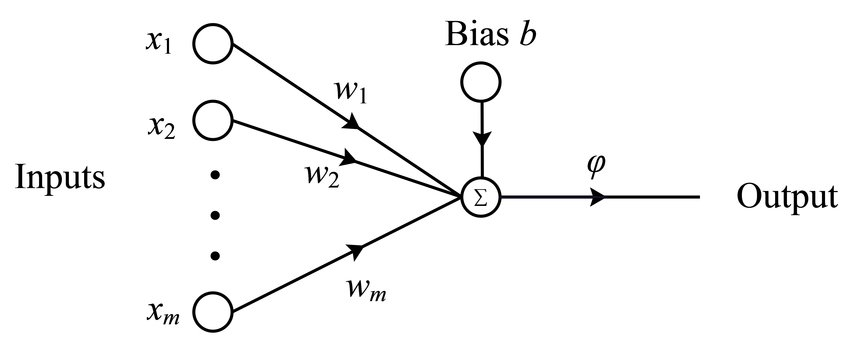
\includegraphics[scale=0.5]{images/fig_chapter2/nns/perceptron.png}
    \caption{Perceptron}
    \label{fig:perceptron}
\end{figure}

\begin{figure}[H]
    \centering
    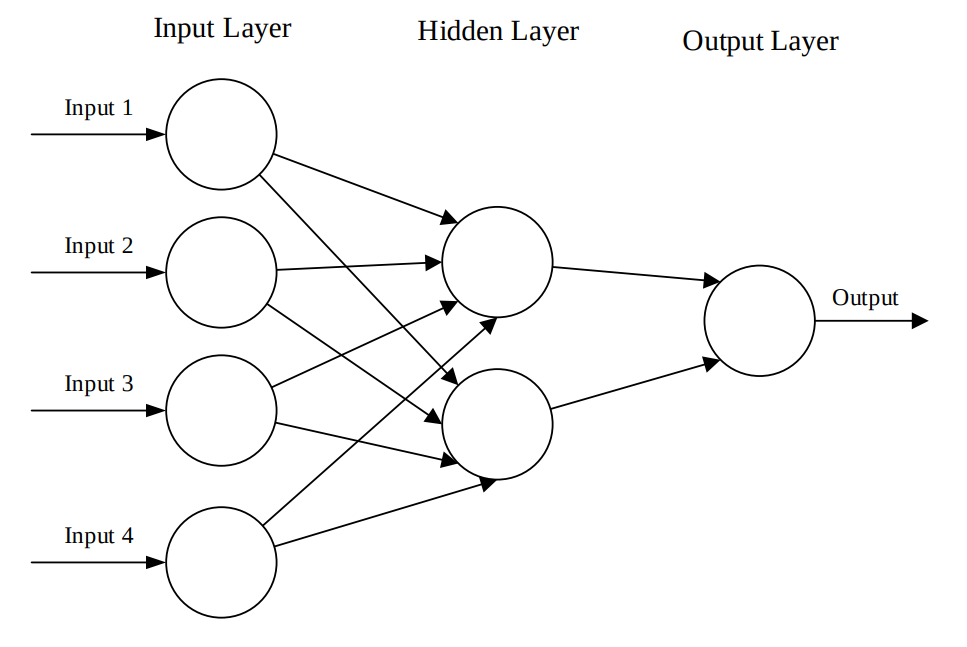
\includegraphics[scale=0.3]{images/fig_chapter2/nns/mlp.png}
    \caption{Multi Layer Perceptron}
    \label{fig:mlp}
\end{figure}

\subsection{Convolutional Neural Networks (CNNs)}
CNNs are another class of ANNs and are responsible for revolutionising the field computer vision and has applications in Natural Language Processing, Recommender Engines and Time Series. These networks also have neurons that self-optimise through learning \citep{cnn2015introduction}. These networks are capable of learning multiple features from the data by abstracting the data into feature maps. In our case we input a 6 channel (3-accelerometer and 3-gyroscope) data and then the CNNs take the data from 6 channels to 64 channels (feature maps). Then these features are fed into the Fully Connected Layers (FC / MLP) at the end to regress the pose as shown in figure \ref{fig:cnn_fc}. This also results in reducing dimensionality of the data while regressing the output. 

\begin{figure}[H]
    \centering
    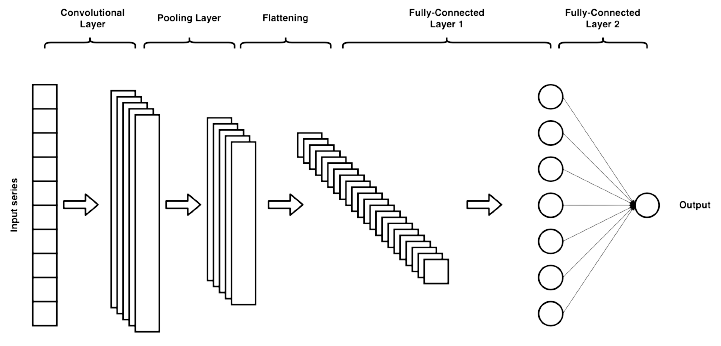
\includegraphics[scale=0.4]{images/fig_chapter2/nns/cnn_mlp.png}
    \caption{CNN layers with FC layers}
    \label{fig:cnn_fc}
\end{figure}

\subsection{Transformers}
Transformer architecture as shown in figure \ref{fig:transformer_arch} is one of the latest proposed neural network architectures that has outperformed its predecessors. Its use mainly started for natural language processing \citep{vaswani2017attention} but was also adopted for computer vision \citep{dosovitskiy2020image}. The use of transformers is also extended for Inertial based Human Activity Recognition (HAR) \cite{shavit2021boosting} and Inertial Navigation \citep{rao2022ctin}. This architecture adopts Multi Headed Attention Mechanism (MHA) \citep{vaswani2017attention} which results in weighing the significance of each part of input data. This significantly improves performance of the network as it learns the importance of each feature and can look at the bigger picture from the data.

\begin{figure}[H]
    \centering
    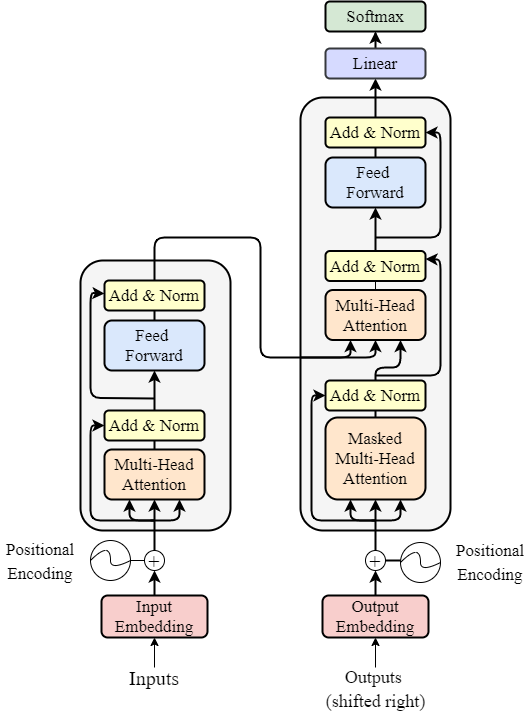
\includegraphics[scale=0.5]{images/fig_chapter2/nns/transformer_arch.png}
    \caption{Transformer Architecture}
    \label{fig:transformer_arch}
\end{figure}

\begin{figure}[H]
    \centering
    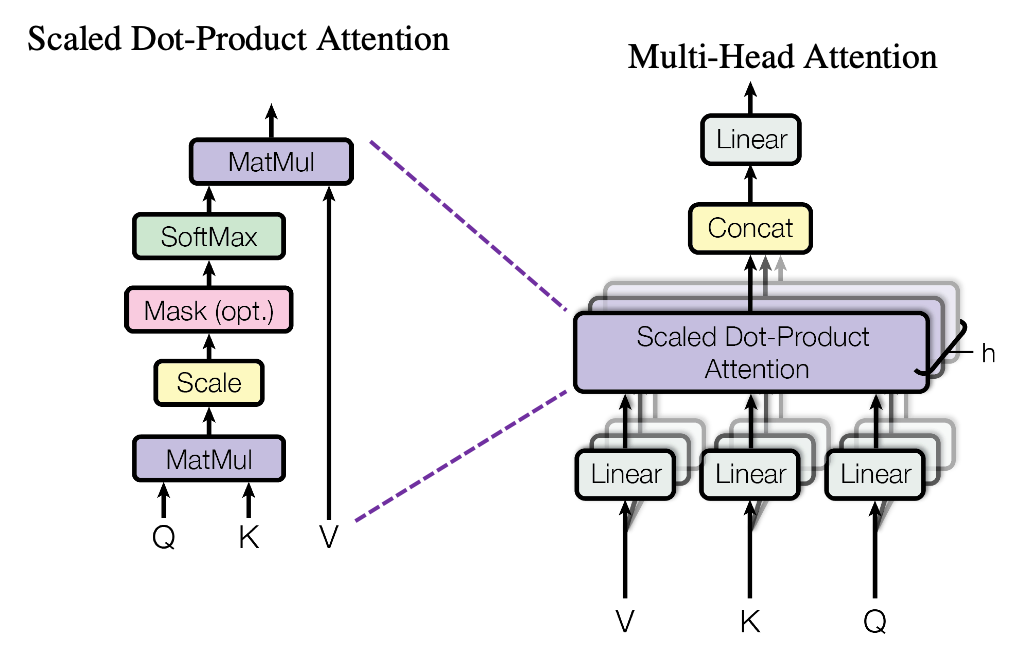
\includegraphics[scale=0.4]{images/fig_chapter2/nns/mha_img_original.png}
    \caption{Multi Headed Attention}
    \label{fig:mha}
\end{figure}

% \begin{figure}[H]
%     \centering
%     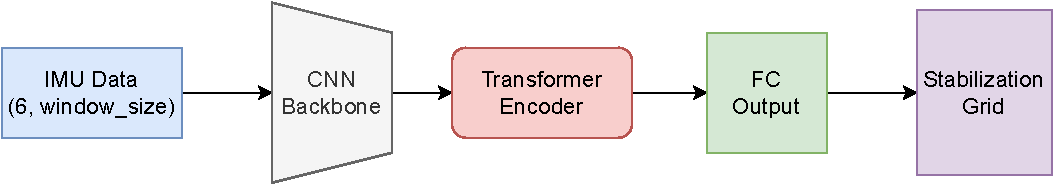
\includegraphics[scale=0.7]{images/fig_chapter2/nns/transformer_cnn.pdf}
%     \caption{CNN-Transformer}
%     \label{fig:transformer_cnn}
% \end{figure}


In this chapter we discussed different methods for image stabilization, challenges of pose-estimation  and which methods are available to estimate pose from MEMS IMUs. The next chapter summaries some state of the art techniques used to solve the challenges we are facing.
